% eec_nrp_dspr.tex       written by M. Comyn       last updated 23-05-2012 by NM

% Use this LaTeX file to submit your TRIUMF EEC New Research Proposal or Progress Report
% Detailed Statement of Proposed Research

% NOTE:
% You must enter your experiment number between the braces of the
% \setcounter{expnum}{}
% command located at the foot of this file, prior to entering your text.

%##########################################################################

\documentclass[12pt]{article}
\usepackage{latexsym,multicol,bm}
\usepackage[pdftex]{graphicx, rotating, color}
\usepackage{amsmath}
\usepackage{amssymb}
\usepackage{dcolumn}
\usepackage{longtable}
\usepackage{pifont}
\DeclareGraphicsRule{.pdftex}{pdf}{*}{}
%\usepackage{blindtext}

% Use Michel Goossens' dense lists Itemize, Enumerate and Description

\let\Otemize =\itemize
\let\Onumerate =\enumerate
\let\Oescription =\description
% Zero the vertical spacing parameters
\def\Nospacing{\itemsep=0pt\topsep=0pt\partopsep=0pt\parskip=0pt\parsep=0pt}
% Redefine the environments in terms of the original values
\newenvironment{Itemize}{\Otemize\Nospacing}{\endlist}
\newenvironment{Enumerate}{\Onumerate\Nospacing}{\endlist}
\newenvironment{Description}{\Oescription\Nospacing}{\endlist}

\newcounter{expnum}

\renewcommand{\thebibliography}[1]{\list
 {\arabic{enumi}.}{\settowidth\labelwidth{[#1]}\leftmargin\labelwidth
 \advance\leftmargin\labelsep
 \usecounter{enumi}}
 \renewcommand{\newblock}{\hskip .11em plus .33em minus -.07em}
 \itemsep=0pt\topsep=0pt\partopsep=0pt\parskip=0pt\parsep=0pt
 \sloppy
 \sfcode`\.=1000\relax}
\let\endthebibliography=\endlist

\makeatletter
\renewcommand{\ps@plain}{%
 \renewcommand{\@oddhead}{\sffamily\bfseries
 \hspace{-2mm}%
 \begin{tabular}[t]{|p{180mm}|}\hline
  {\footnotesize
  TRIUMF EEC New Research Proposal
  \hspace{\fill}
  Detailed Statement of Proposed Research for Experiment \#: \theexpnum}\\ \hline
 \rule[-242mm]{0mm}{0mm}\\ \hline
 \end{tabular}}
 \renewcommand{\@evenhead}{\@oddhead}
 \renewcommand{\@oddfoot}{\sffamily\hfil\thepage\hfil}
 \renewcommand{\@evenfoot}{\@oddfoot}}
\makeatother

\textwidth      180mm
\textheight     240mm
\topmargin      -20mm
\oddsidemargin   -7mm
\flushbottom
\frenchspacing

\pagestyle{plain}

\begin{document}

\footnotesize\sffamily

\noindent
\textbf{The EEC committees strongly recommend that you limit your
submissions, including figures and tables, to no more than 4 pages for the
MMSEEC or 10 pages for the SAPEEC. \ The following information should be
included:}\\

\scriptsize\sffamily

% \begin{Itemize}
% \item[(a)]
% \textbf{Scientific value of the experiment:}
% Describe the importance of the experiment and its relation to previous
% work and to theory.  All competitive measurements at other laboratories
% should be mentioned.  Include examples of the best available theoretical
% calculations with which the data will be compared.
% \item[(b)]
% \textbf{Description of the experiment:}
% Techniques to be used, scale drawing of the apparatus, measurements to be
% made, data rates and background expected, sources of systematic error,
% results and precision anticipated.  Compare this precision with that
% obtained in previous work and discuss its significance in regard to
% constraining theory.  Give a precise list of targets to be used in order of
% their priority.
% \item[(c)]
% \textbf{Experimental equipment:}
% Describe the purpose of all major equipment to be used.
% \item[(d)]
% \textbf{Readiness:}
% Provide a schedule for assembly, construction and testing of equipment.
% Include equipment to be provided by TRIUMF. For secondary beam for ISAC, provide information on established yields of the isotope of interest as well as the established isobaric contaminants form the same target/ion-source combination.
% \item[(e)]
% \textbf{Beam time required:}
% State in terms of number of 8-hour shifts.  Show details of the beam time
% estimates, indicate whether prime-user or parasitic time is involved, and
% distinguish time required for test and adjustment of apparatus.
% \item[(f)]
% \textbf{Data analysis:}
% Give details and state what data processing facilities are to be provided
% by TRIUMF.
% \end{Itemize}

\footnotesize\sffamily

\normalsize\rmfamily

%##########################################################################

\setcounter{expnum}{1754} %Enter your experiment number between the braces

%##########################################################################

% Enter Detailed Statement of Proposed Research below:
\noindent\textbf{(a) Scientific value of the experiment:}
%\section{Scientific value of the experiment}
%Describe the importance of the experiment and its relation to previous
%work and to theory.  All competitive measurements at other laboratories
%should be mentioned.  Include examples of the best available theoretical
%calculations with which the data will be compared.

It is our goal to simultaneously perform cyclotron frequency measurements and collinear laser spectroscopy on odd-A cadmium nuclei from $^{123-129}$Cd. This proposal represents the first step in a campaign of concurrent measurements of short-lived nuclei with isomeric states of comparable lifetimes as a means of definitively assigning energy, spin, and parity in regions of the chart of nuclides where definitive assignments based on theory and systematics are not credible. As of this moment there is no competitive method for the assignment of these states.

\begin{figure}[ht]
    \begin{center}
        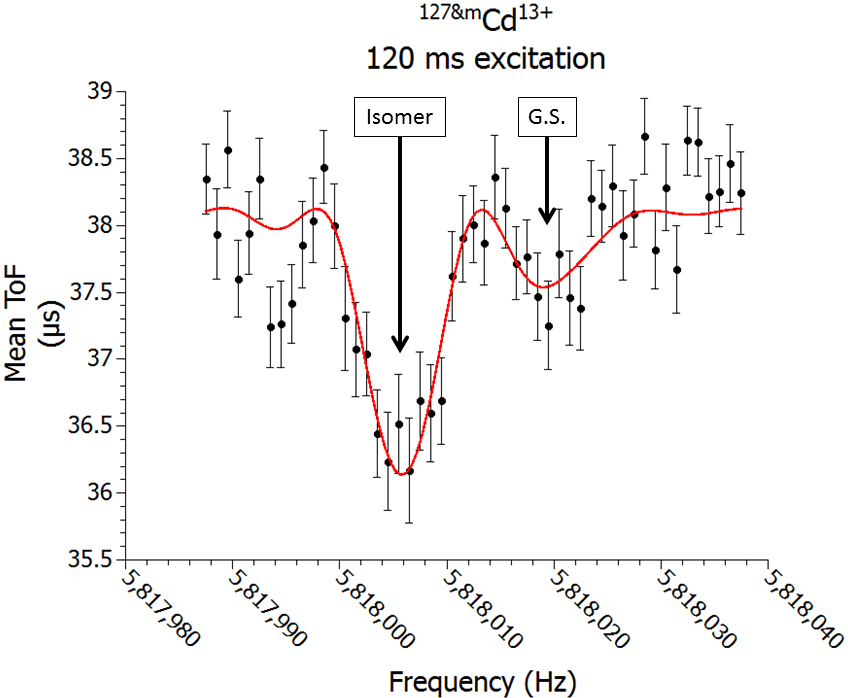
\includegraphics[width=0.5\textwidth]{127Cd.png}
        \caption[$^{127}$Cd ToF Spectrum]{One of the Time-of-Flight resonance spectra from the recent measurement of the mass of $^{127}$Cd \cite{Lascar2017}. Both the ground state (shallower trough) and the isomeric state (deeper trough) are visible and the state with the deeper trough is the one with the greatest abundance inside the Penning trap.}
        \label{fig:127Cd}
    \end{center}
\end{figure}

Recent investigations by the TITAN group and TRIUMF-based theorists \cite{Lascar2017} have demonstrated the insufficiency of systematic arguments in assigning spin and parity for the ground and isomeric state in odd-A Cd nuclei. In precisely measuring the masses of $^{125g/m}$Cd and $^{127g/m}$Cd (including the the first measurement able to differentiate the ground and isomeric state masses in $^{127}$Cd which can be seen in Figure \ref{fig:127Cd}) we were able to determine the energy separation between the respective ground states and their isomers. However, Penning trap mass spectrometry cannot assign spins and parities to the observed states, limiting comparisons with theoretical models.

\begin{figure}[ht]
    \begin{center}
        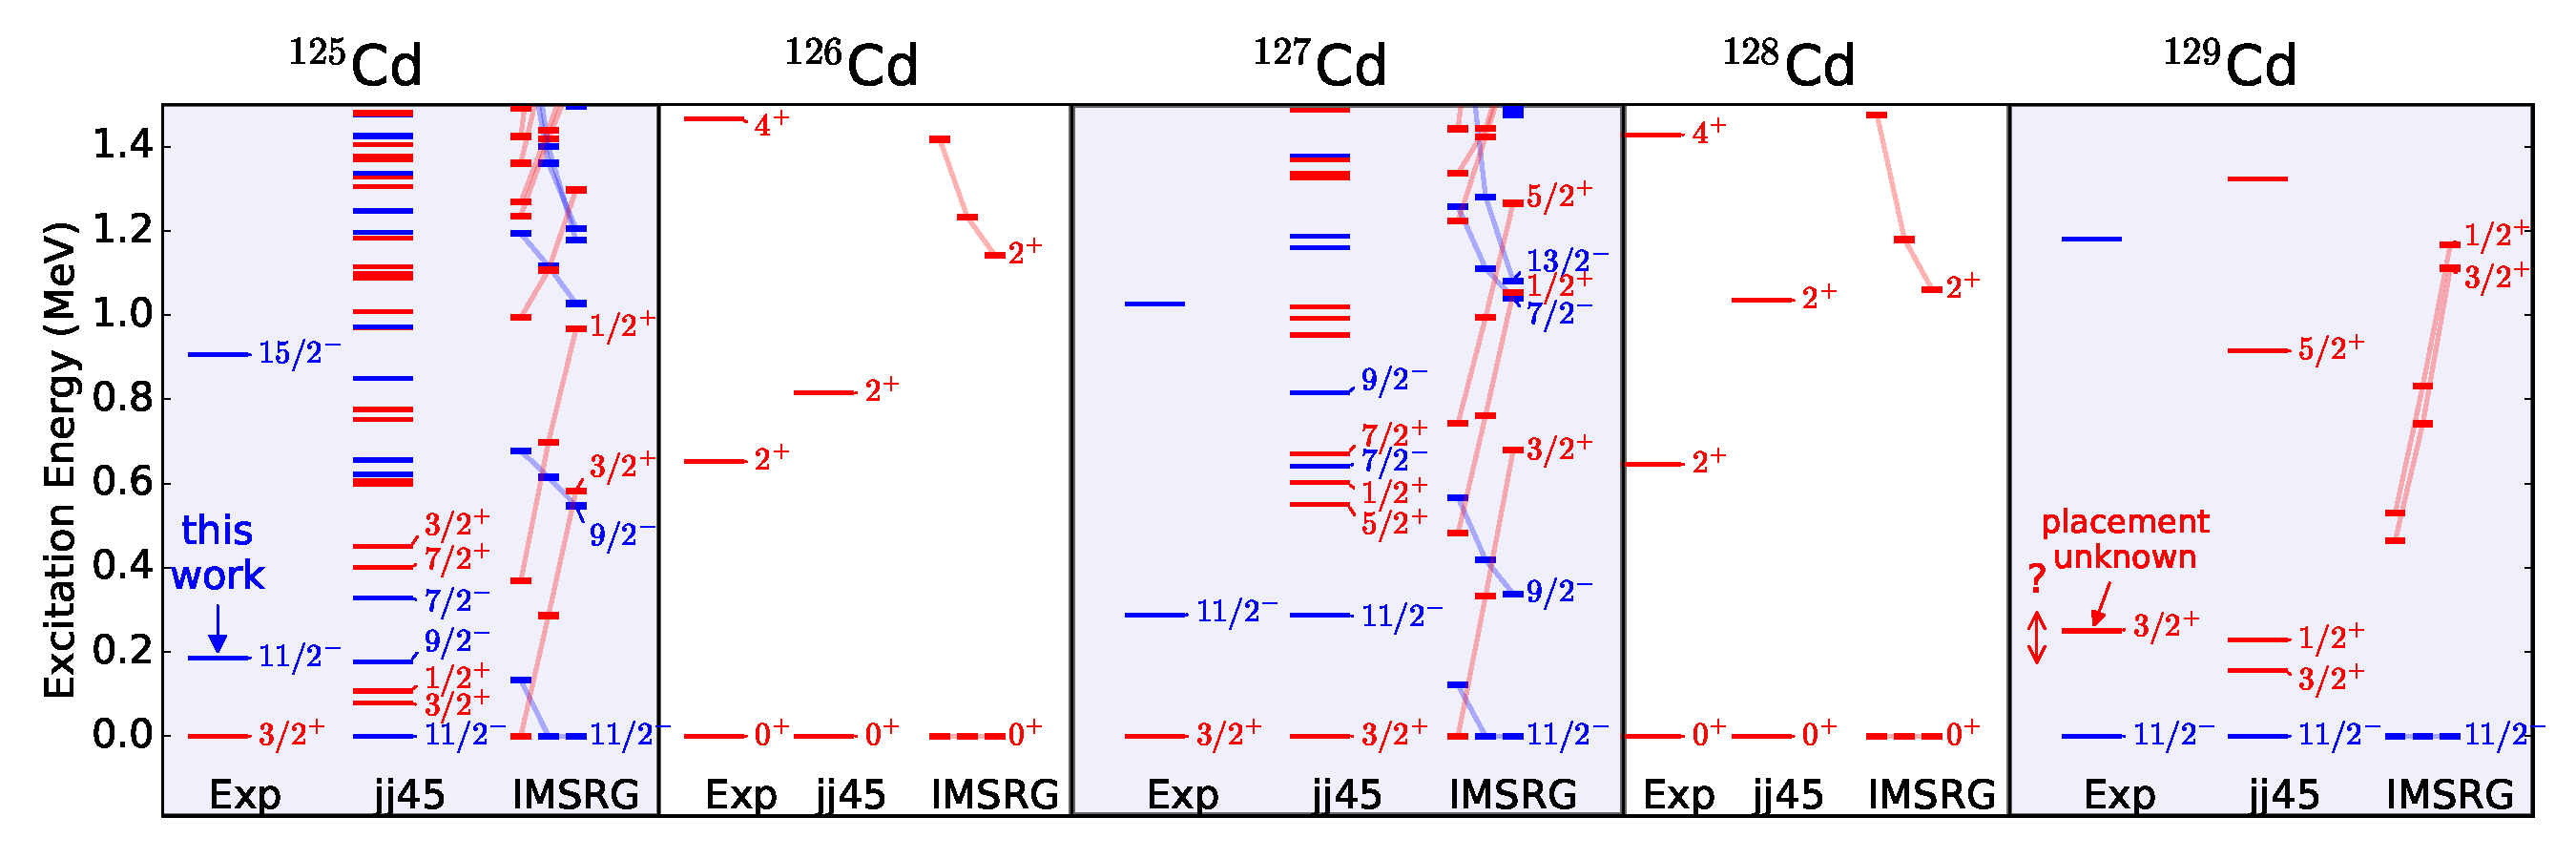
\includegraphics[width=\textwidth]{Cd_spectra_v2.pdf}
        \caption{Experimental level schemes for $^{125-129}$Cd compared with phenomenological shell-model predictions using the jj45 interaction \cite{Dillmann2003} and {\it ab initio} results obtained with the valence-space IMSRG \cite{Tsukiyama2012,Bogner2014,Stroberg2016,Stroberg2017}. Experimental values from outside \cite{Lascar2017} were taken from the National Nuclear Data Center \cite{NNDC2016}. Positive parity states are indicated with red lines while negative parity states are indicated with blue lines. Black lines indicate unknown parity. The energy of the $3/2^+$ state in $^{129}$Cd relative to the $11/2^-$ state is unknown experimentally and so its placement in the level scheme is arbitrary. The IMSRG results display a series of $e_{\mathrm{max}}/E_{3\mathrm{max}}$ truncations (from left to right) 14/14, 14/16, 14/18 (see text for details). No indication of convergence [was] observed. Figure and caption reproduced from \cite{Lascar2017}.}
        \label{fig:level}
    \end{center}
\end{figure}

The vast majority of spin and parity assignments of neutron-rich cadmium nuclei are made via systematic arguments and comparison with shell-model calculations \cite{ENSDF}. In verifying this for a recent publication \cite{Lascar2017}, the authors performed several shell model and \emph{ab initio} calculations. The shell-model calculations were performed with the NuShelX shell-model code \cite{Brown2003} using the jj45 effective interaction \cite{Dillmann2003}, while the \emph{ab initio} calculations were performed using the valence space In-Medium Similarity Renormalization Group (IMSRG) approach \cite{Tsukiyama2012,Bogner2014,Stroberg2016,Stroberg2017}. Figure \ref{fig:level} shows the results of these calculations.

The jj45-calculated levels show ground state spins alternating between $11/2^-$ and $3/2^+$ with increasing neutron number in the odd-A, neutron-rich Cd nuclei. The IMSRG calculations failed to show convergence on either absolute binding energies or relative excitation energies. 

Several collinear laser spectroscopy experiments by Yordanov \emph{et al.} at ISOLDE \cite{Yordanov2013,Yordanov2016} have looked at the neutron-rich cadmium region specifically. They were able to elegantly identify the existence of states but ordering those identified states was again based on systematic arguments.

Still, the collinear laser spectroscopy experiment points to a means of definitive assignment if used in conjunction with a Penning trap mass measurement. While collinear laser spectroscopy cannot, on its own, determine the ordering of the states observed it can determine the relative abundance of the observed states. If an ion bunch, identically composed to the one sent to the collinear laser spectroscopy experiment, was sent to a Penning trap experiment for mass measurement then along with measuring the energies of the ground state and isomers, the relative depths of the troughs in a Penning trap mass measurement spectrum (see Figure \ref{fig:127Cd}) would be a measure of the relative abundance of the observed states.

Thus, a collinear laser spectroscopy experiment operating in concert with a Penning trap mass measurement experiment could definitively assign spin, parities, and energies to nuclei with long lived isomeric states. All that is required is an identical beam sent to both experiments.

TRIUMF is well positioned to make these measurements because the TITAN RadioFrequency Quadrupole cooler/buncher (RFQ discussed below) is an integral part in both TRIUMF's collinear laser spectroscopy experiment and TITAN's Penning trap mass measurement experiment. The RFQ sends bunched beams to both experiments \cite{Brunner2012a} and would be an integral part in ensuring an identical ion bunch sent to each experiment. Similar setups exist at ISOLDE with ISOLTRAP \cite{Bollen2001} and COLLAPS \cite{Papuga2014}, and at Jyv\"{a}skyl\"{a} with JYFLTRAP \cite{Kolhinen2004} and the IGISOL collinear laser spectroscopy experiment \cite{Billowes2000}\footnote{Which, sadly, lacks a clever acronym.}. To our knowledge there is no attempt to perform these concurrent measurements at this time.

Narrowing this group down further by facilities with a demonstrated capability of producing and observing neutron-rich Cd leaves ISOLTRAP/COLLAPS as potential direct competitors but to our knowledge, there are no plans for either experiment to revisit neutron-rich Cd before the planned 2018 extended ISOLDE facility shutdown. Performing the experiment now will give TRIUMF a major advantage in these types of measurements.\\

\noindent\textbf{(b1)Description of the experiment:} Penning Trap

%\section{Description of the experiment}
%Techniques to be used, scale drawing of the apparatus, measurements to be
%made, data rates and background expected, sources of systematic error,
%results and precision anticipated.  Compare this precision with that
%obtained in previous work and discuss its significance in regard to
%constraining theory.  Give a precise list of targets to be used in order of
%their priority.
\begin{figure}[ht]
    \begin{center}
        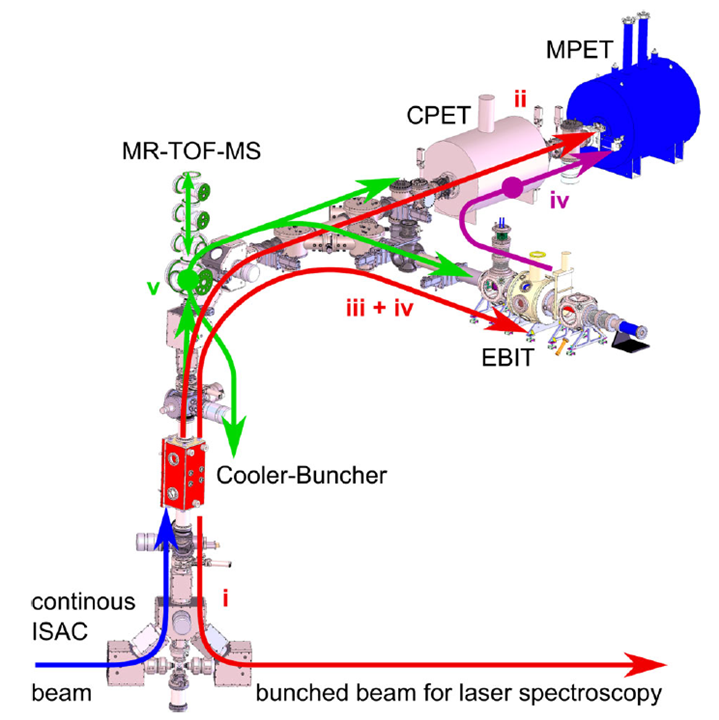
\includegraphics[width=10cm]{TITAN_MRTOF.png}
        \caption[The TITAN experiment]{An overview of the TITAN experiment. Beam is bunched in the RFQ. SCI bunches go to MR-ToF for mass separation before being sent to the EBIT for charge breeding. SCIs from the RFQ or HCIs from the EBIT are sent to MPET for precision mass measurements.}
        \label{fig:TITAN}
    \end{center}
\end{figure}
We propose to measure the cyclotron frequencies and relative abundances of $^{123,125,127,129}$Cd and their respective isomers in a precision Penning trap. TRIUMF's Ion Trap for Atomic and Nuclear science (TITAN) has been performing mass measurements since 2007 \cite{Dilling2003,Dilling2006,Ettenauer2010,Gallant2012}.

Nuclides of interest are produced in the ISAC facility. For the beams requested, ISAC has observed the yields illustrated in Table \ref{table:yields}.

\begin{table}[ht]
\centering
\begin{tabular}{|l|c|c|}
\hline
Species & Proton & ISAC/IG-LIS Yield (\emph{Predicted}) \\
& Current & \\
& ($\mu$A) & ($s^{-1}$) \\
\hline
$^{123}$Cd & 9.8 & $3.9 \times 10^5$ ($\mathit{3.9 \times 10^4}$) \\
$^{123m}$Cd & 9.8 & $9.4 \times 10^5$ ($\mathit{9.4 \times 10^4}$) \\
\hline
$^{125}$Cd & 9.8 & $1.5 \times 10^5$ ($\mathit{1.5 \times 10^4}$) \\
$^{125m}$Cd & 9.8 & $5.8 \times 10^4$ \\
\hline
$^{127}$Cd & 9.8 & $4.8 \times 10^3$ \\
$^{127m}$Cd & 9.8 & $>4.8 \times 10^3$ \\
\hline
$^{129}$Cd & 9.8 & $3.8 \times 10^2$ \\
$^{129m}$Cd & 9.8 & $\sim 10^2$ \\
\hline
\end{tabular}
\caption{Cd production from the ISAC yield database. $^{123/m}$Cd were produced with a UO target and the remainder were produced with a UCx target. Where yields were produced by the IG-LIS source, the yield is in plain text. Where the yields were produced by the FEBIAD source, the FEBIAD value is given in plain text and the \emph{italicized} text is the predicted yield via IG-LIS assuming an order of magnitude reduction in yield.}
\label{table:yields}
\end{table}

Nuclides produced in ISAC are sent to TITAN's RadioFrequency Quadrupole (RFQ) gas-filled trap which accepts ISAC's continuous 20 keV beam for cooling and bunching. They are then mass separated in the recently commissioned TITAN Multi-Reflection Time-of-Flight mass spectrometer (MR-ToF) \cite{Jesch2015} which oscillates the ions back and forth between two electrostatic mirrors and separates masses at the isobaric level simply via their times-of-flight after $\sim 10^2$ oscillations.

The cooled, bunched beam is ejected at $\sim$2 keV and transported to TITAN's Electron Beam Ion Trap (EBIT) for charge breeding before being sent to TITAN's Measurement PEnning Trap (MPET). In the EBIT, a DC trap confines the ions axially while a tunable magnetic field\footnote{6 T maximum but recently run at $\sim 4$ T \cite{Klawitter2015}.} confines the ions radially. An energetic electron beam is fired into the confined ion bunch. The electron beam strips bound electrons from the trapped ions and the final charge state of the ion is a function of the electron beam's energy, the electron beam's current density, and the charge breeding time ($t_b$) spent in the EBIT \cite{Froese2006}. The use of the EBIT to make these measurements was demonstrated in \cite{Lascar2017} and was, in fact, critical in creating a sufficient separation between the ground state and the isomer in the frequency space available.

In MPET, the ions are confined radially via a 3.7 T, uniform magnetic field and axially via a harmonic potential created by electrodes that essentially form two hyperboloids of revolution\footnote{Plus some correction electrodes to compensate for the missing material in the main hyperbolic trap electrodes.}. 

% In a uniform magnetic field, an ion will orbit at the cyclotron frequency
% \begin{equation}
% \omega_c = \frac{qB}{m}
% \end{equation}
% where $B$ is the magnetic field, $q$ is the ion's charge and $m$ it's mass. The addition of the axial harmonic electrostatic potential splits $\omega_c$ into two eigenmotions: the smaller, ``magnetron'' motion, $\omega_{-}$ with frequencies $\approx 6$ kHz and the larger, ``reduced cyclotron'' motion, $\omega_{+}$ with frequencies $\sim \omega_c \sim 5$ MHz (for an $A/q$ of 9.25). In a hyperbolic Penning trap (such as MPET), the two eigenmotions are related by
% \begin{equation}
% \omega_c = \omega_{+} + \omega_{-}.
% \end{equation}

TITAN measures the cyclotron frequency, $\nu_c$ using the well established ToF-ICR method \cite{Brown1982b}.

The precision achievable by a given measurement is
\begin{equation}
\frac{\delta m}{m} = \frac{m}{qB}\frac{C}{t_{\mathrm{RF}}\sqrt{N}}
\label{eq:precision}
\end{equation}
where $C$ is a dimensionless quantity that depends on the quality of the fit made by the fitting function as well as the purity of the sample of the ions in the trap (and should be approximately equal to 1). $t_{\mathrm{RF}}$ is the time that the quadrupole excitation was applied and should be set to roughly twice the half-life of the ion being measured. $N$ is simply the number of ions of interest observed over the course of the measurement.

Contaminant ions can be resonantly excited via a dipole excitation at the contaminant's reduced cyclotron frequency. A resonant dipole excitation will increase the ion's orbital radius and the goal, in this case, is to increase the radius such that:
\begin{enumerate}
\item The contaminants don't interfere with the ion being probed with the quadrupole excitation.
\item When the trap is opened after the excitations are complete, the orbital radius will be larger than the aperture at the end of the trap so the contaminants hit the trap walls and not the MCP.
\end{enumerate}

Normally, when making a precision mass measurement TITAN would be interleaving these measurements with measurements of a calibrant ion of well known mass. Given that these Cd ground state and isomeric masses were recently measured to high precision \cite{Lascar2017,Hakala2012,Kankainen2013,Atanasov2015} there is no need for a full mass measurement. Instead, we propose to simply measure the cyclotron frequencies of the isomer and the ground state as we did in Figure \ref{fig:127Cd}. In that figure, both states can be readily observed, are obviously identifiable, and are produced at different rates. The relative yields of each state will then be compared to those observed using collinear laser spectroscopy to unambiguously determine the ground- and isomeric-state spins and parities.\\

\noindent\textbf{(b2)Description of the experiment:} Laser spectroscopy

Collinear laser spectroscopy has been the workhorse of laser spectroscopy at radioactive beam facilities for many years \cite{Campbell2016}. The basic experimental arrangement is shown in figure \ref{colfig}.
\begin{figure}
\begin{center}
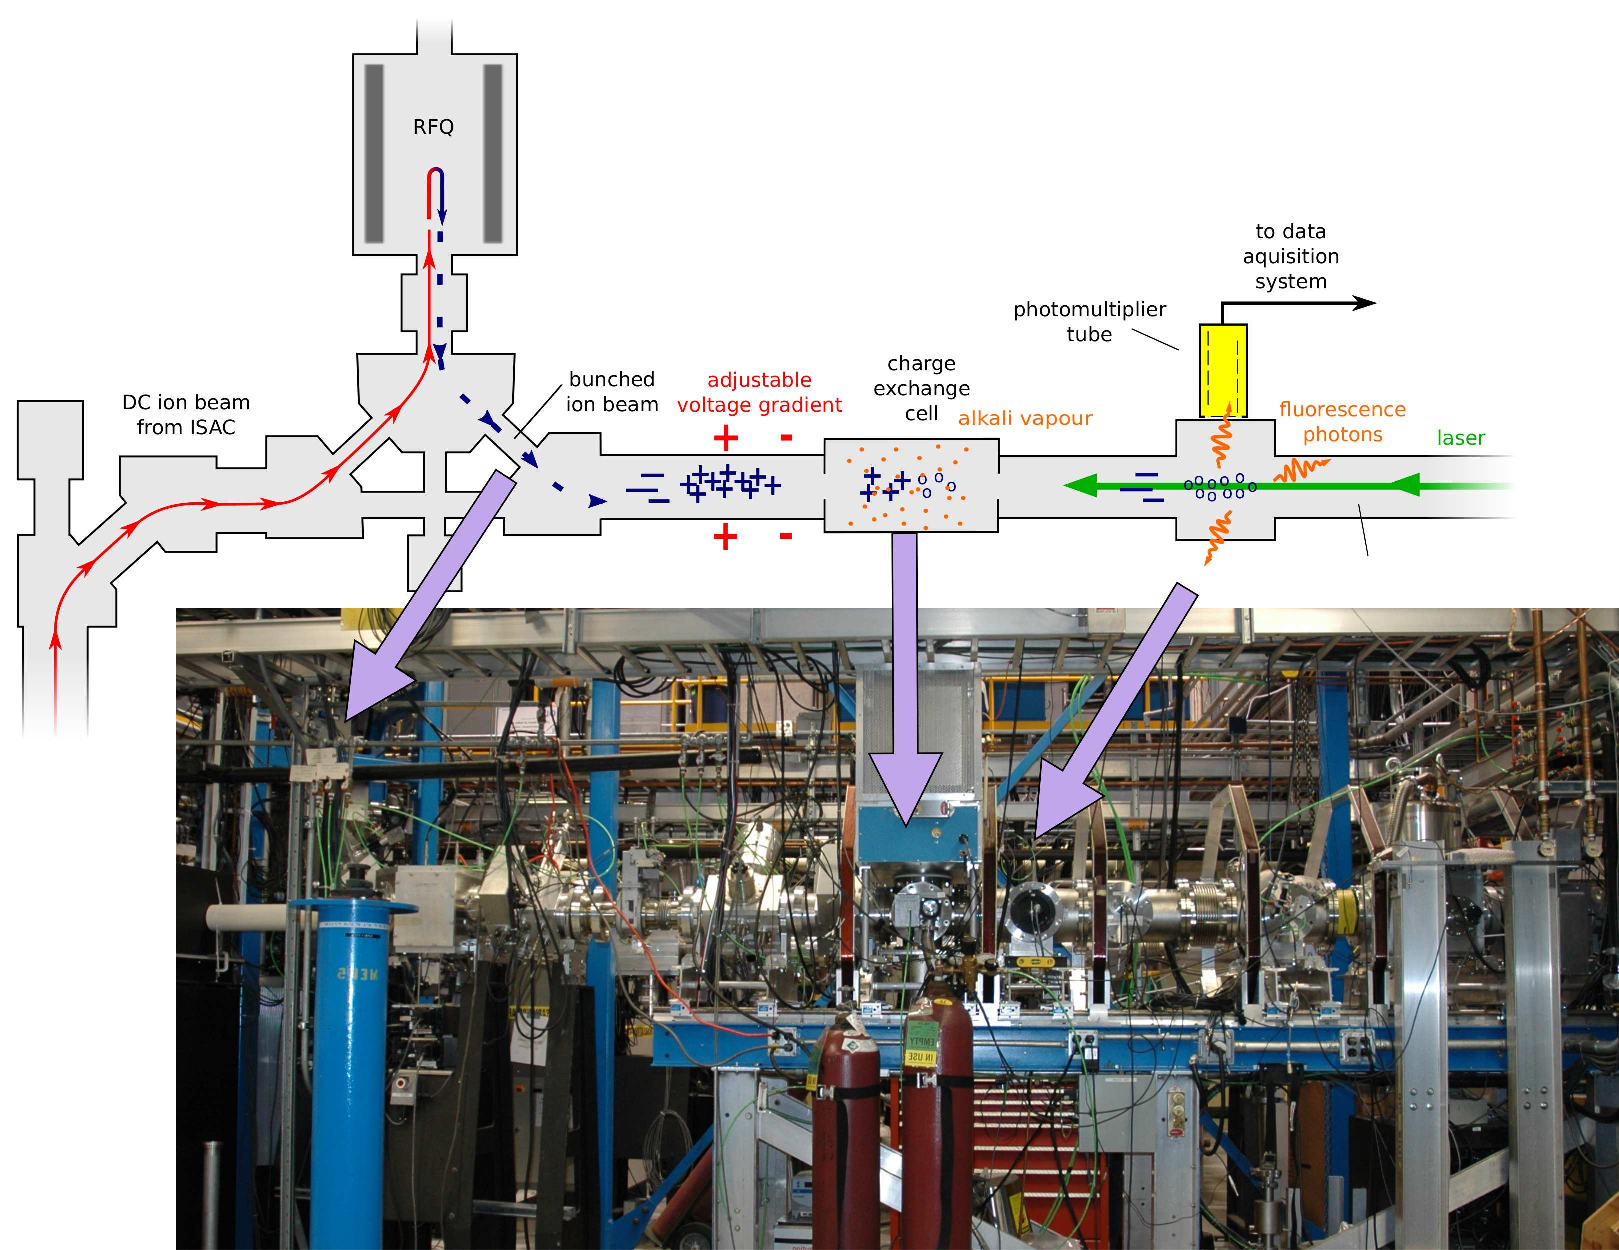
\includegraphics[height=3in]{beam-RFQ.pdf}
\caption{The collinear experimental set-up at \textsc{Triumf}}\label{colfig}
\end{center}
\end{figure}

The overlapping of a laser and ionic beam leads to a high probability of excitation and subsequent re-emission of absorbed photons if the frequency of the laser as seen in the reference frame of the ion matches that of an allowed atomic transition. A fast beam is used so as to compress the velocity spread of the beam inherent from any hot ion source allowing  high precision, almost Doppler-free spectroscopy to be performed. As the laser frequency of interest is not the frequency of the laser in the lab frame but that in the rest frame of the fast ion beam it is possible to scan the laser frequency across the atomic transition by either scanning the laser frequency or by changing the velocity of the ion beam. The latter is in general the preferred system as it offers most flexibility as well as  reproducibility.

Cd offers the possibility of being probed either on the atom or ion. The relevant electronic structure is shown in figure \ref{fig:cdelectronic} along with the wavelengths required for non-resonant ionization from the excited states in the  atom. Detailed investigations into the structures of all the nuclear states of interest to this proposal have already been studied using the ionic transitions at CERN \cite{Yordanov2013,Yordanov2016}. Therefore spectroscopy at the level required for extraction of properties is not needed, the only requirement is that the different states are identifiable from each other.
%\begin{figure}
%\begin{center}
%\resizebox{3in}{!}{\input{cdiandii.pdftex_t}}
%\caption{Relavent electronic structure of Cd atom (left) and ion (right)}
%\label{fig:cdelectronic}
%\end{center}
%\end{figure}

\begin{figure}
\begin{center}
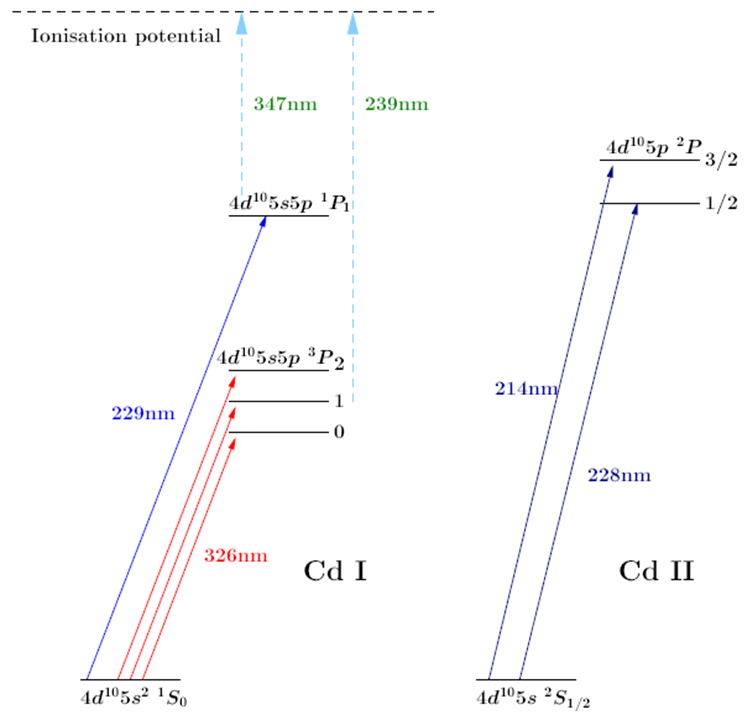
\includegraphics[width=7cm]{e_structure.png}
\caption{Relevant electronic structure of Cd atom (left) and ion (right)}
\label{fig:cdelectronic}
\end{center}
\end{figure}

Based on the data in Table \ref{table:yields}, this proposal requests the use of the Uranium Carbide target and the IG-LIS source as it produced beams with contaminants suppressed by up to 5 orders of magnitude relative to the beam of interest. Beamtime requests are in Section \emph{e} below.\\

\noindent\textbf{(c) Experimental equipment:}
%\section{Experimental equipment}
%Describe the purpose of all major equipment to be used.
TITAN will use the following four devices to make the measurements.
\begin{itemize}
\item The RFQ: TITAN accepts continuous beam from ISAC via a RadioFrequency Quadrupole (RFQ) trap. The RFQ thermalizes the 20 keV ISAC beam via its He gas. The trap bunches the beam to single eV/q energies. The bunch is extracted at $\sim$ 2 keV for transport down the beamline to the EBIT.

\item The TITAN MR-ToF: In May TITAN successfully commissioned an MR-ToF mass spectrometer with a mass resolution ($m/\Delta m$) of greater than 200,000. Ions are mass speparated via their times-of-flight after undergoing many ($\sim 10^2$) turns between two electrostatic mirrors at either end of the MR-ToF's analyzer.

\item MPET: TITAN's Measurement PEnning Trap (MPET) is the precision Penning trap where mass measurements are made. Ions are confined radially in MPET's 3.7 T magnetic field and then confined axially via the harmonic potential created by its hyperbolic electrodes. A trapped ion's cyclotron frequency is measured via the Time of Flight Ion Cyclotron Resonance (ToF-ICR) method and from there the mass is calculated.

\item The EBIT: TITAN's Electron Beam Ion Trap is used to charge breed ions from the RFQ. Charge breeding the ion increases the precision as a smaller $A/q$ yields a higher measured frequency, $\omega_c$, and thus a smaller $\frac{\delta \omega}{\omega}$. The final charge state of the bunch trapped in the EBIT is a function of both the electron beam current and the time spent in the trap. Once the ions have been charge bred, the charge state is selected from its ToF via a Bradbury-Nielsen Gate (BNG) on its way towards MPET.

    %Equation \ref{eq:gain} defines the requirements for using the EBIT in order to realize precision gains from charge breeding.
    Charge breeding times for various Cs charge states can be seen in Fig. \ref{fig:charge_breeding}. A charge state of 7+ is sufficient to yield precision gains and from TITAN's experience \cite{Ettenauer2013,Klawitter2015} a charge state of $15^+$ or $16^+$ is the largest that will survive in MPET's vacuum to make a sufficient measurement.

    \begin{figure}[ht]
        \begin{center}
        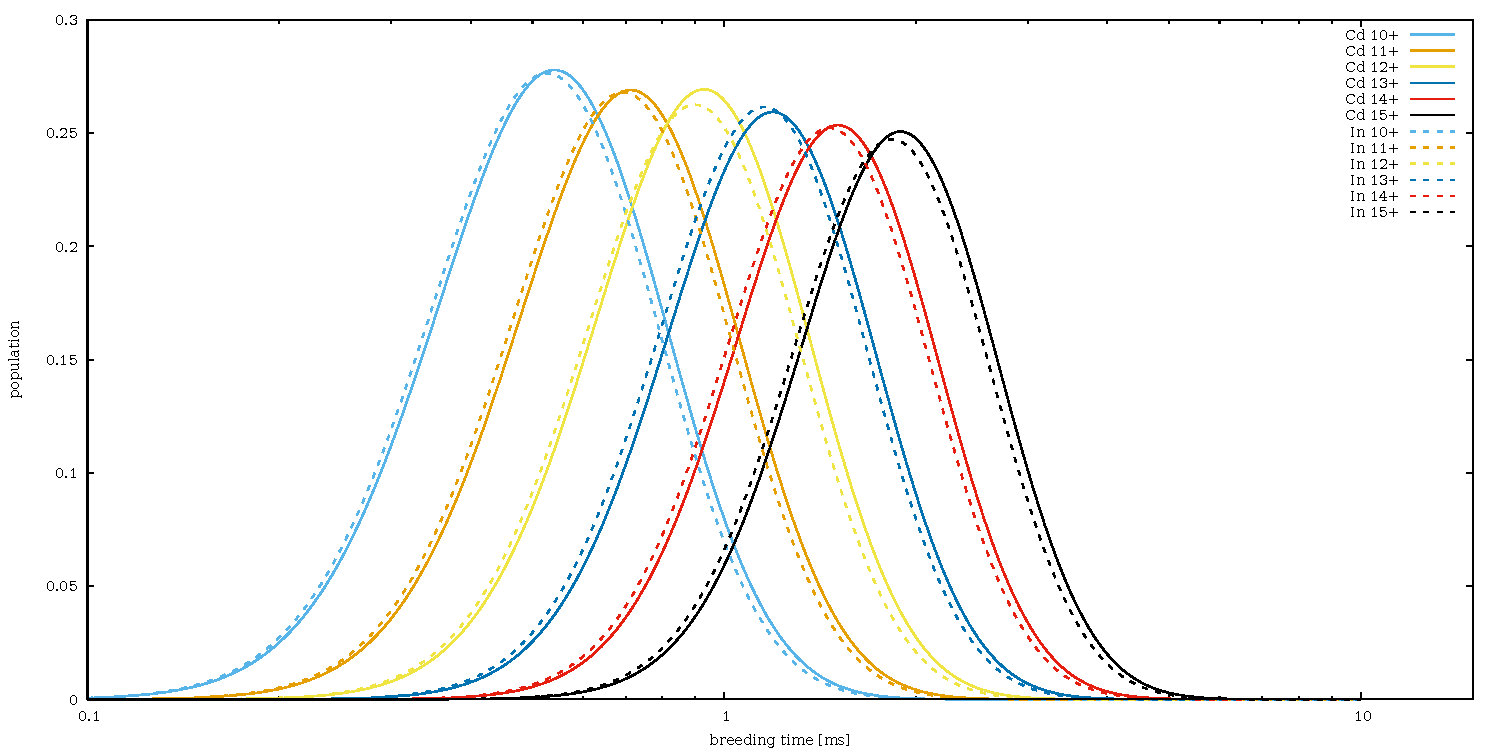
\includegraphics[width=13cm]{for_dan.pdf}
        \caption[Cd Charge Breeding]{The population fraction vs. charge breeding time for $^{127}$Cd and $^{127}$In for charge states $10^{+}$ to $15^{+}$. Calculations performed by R. Klawitter.}
        \label{fig:charge_breeding}
        \end{center}
    \end{figure}

\end{itemize}

The laser spectroscopy experiment will use the following equipment to make their measurements:

\begin{description}

\item [\textsc{Titan}'s RFQ]  Continuous beams will be taken from \textsc{Isac} and bunched in an identical manner to that described for the mass meansurements above. The bunched beam will then be reverse ejected back in to the low energy beam transport section of \textsc{Isac} and directed towards the polariser line.

\item [Polariser line] \textsc{Triumf}'s polariser line has been in operation for both laser spectroscopy and laser induced polarisation of radioactive beams for many years. Dependent upon the detection scheme decided upon it will be configured in one of two ways.

\begin{description}
\item [Fluorescence detection on Cd$^+$]  This is the classical collinear laser spectroscopy detection technique, used in multiple experiments with this setup \cite{Voss2016}. Narrow linewidth single mode laser light at 214nm will be overlapped collinearly with the bunched ion beam. These will both pass through a novel spherical  mirror assembly that is floatable in electrical potential. This potential is then swept in order to Doppler tune the frequency of laser light in the rest frame of the ion. The resulting fluorescence will be observed by a photomultiplier tube. For the very low intensity beams background reduction could be further achieved by detecting the ions as well as the photons and performing a coincidence.

\item [Resonance ionization detection on Cd atoms]  The ions will first pass through a charge exchange cell, most probably loaded with Rb, that is floatable in voltage. Changing the potential applied to the cell will vary the velocity of the resultant atomic beam, hence Doppler tuning the laser frequencies. Un-neutralized ions are then swept into a beam dump by means of an electrostatic deflector. Two lasers will then be overlapped with the atom beam. A narrow linewidth laser will be used to optically pump the atoms with the required precision, and a second high powered pulsed laser will be used to ionize the Cd atoms from the excited atomic state. The ionized Cd will then be detected off axis using electrostatic deflectors.

\end{description}
\item [Laser systems] Depending upon the scheme utilized one of two laser systems will be used.

\begin{description}

\item [Laser system for fluorescence detection from Cd ions] This requires light at 214nm which will be produced from the fourth harmonic of a Titanium sapphire laser. This laser and the two doubling units required are currently located within the laser spectroscopy laboratory in ISAC I. Unfortunately it is not possible to transport light of such a short wavelength from this laboratory to the beamline. Therefore the intent is to produce light at 428nm within the laboratory and transport this light to the end of the beamline via existing optical fibers where the second doubling unit required to produce the 214nm light will be located. Minimal optics will then be required to shape and transport the 214nm light through the short distance in the air to the beamline.

\item [Laser system for ion detection from Cd atoms] Here frequency doubled light from a dye laser is required as well as a high power, short pulsed frequency quintupled Nd:YAG laser.  The frequency doubled dye laser will be borrowed from the polarizer line with the light being directed via an existing air transport path from that laser. The ionization laser will be a new acquisition that is currently being investigated. Something along the lines of a CryLaS FQSS 213-50 system is envisioned which can be housed within the laser light enclosure at the end of the beamline within the \textsc{Isac} experimental hall.

\end{description}

\item [Data acquisition system] The laser spectroscopy group at \textsc{Triumf} pioneered the use of time resolved data acquisition systems for laser spectrosocpy on radioactive beams. This system is available and ready for use.

\end{description}

\textbf{A comment on the ratio between the ground and isomeric states}\\
\\
The expected ratios between the isomer and the ground state should be between 2:1 and 5:1 (isomer:g.s) using the data from the recent publication \cite{Lascar2017}. Should the ratio be smaller than 2:1 and approach unity, a retune of the source lasers will change the ratio in favor of one state.


\noindent\textbf{(d) Readiness:}
%\section{Readiness}
%Provide a schedule for assembly, construction and testing of equipment.
%Include equipment to be provided by TRIUMF. For secondary beam for ISAC, provide information on established yields of the isotope of interest as well as the established isobaric contaminants form the same target/ion-source combination.


All required experimental equipment associated with TITAN is prepared for the experiment. TITAN has shown repeated ability to make measurements such as these \cite{Gallant2012a,Simon2012,Ettenauer2011,Lapierre2012,Frekers2013,Ettenauer2013,Klawitter2015,Lascar2017}.

In terms of contaminants, Cs and In were the most dominant and required cleaning in MPET via the dipole excitation of their reduced cyclotron frequencies. The use of the now commissioned MR-ToF should obviate the need for cleaning in MPET but the capability will remain in place.

From TRIUMF, TITAN would require the use of the ISAC yield station prior to the measurement in order to determine the beam rate and the relative concentration of contaminants it may contain.

For the laser spectroscopy experiment the majority of the hardware is currently available on site, and the necessary expertise is in place to implement all the techniques discussed above. The one item that requires purchasing is an off-the-shelf laser system to accomplish the ionization of Cd from the excited state.  Significant development is needed in order to investigate the atomic structure of the ground state and reliably obtain the laser frequencies required. However, it is expected that this can take place on a timescale that is conducive with this proposal.\\

\noindent\textbf{(e) Beam time required:}
%\section{Beam time required}
%State in terms of number of 12-hour shifts.  Show details of the beam time
%estimates, indicate whether prime-user or parasitic time is involved, and
%distinguish time required for test and adjustment of apparatus.

To test the laser excitation schemes before performing this experiment with RIB, we request two days (\emph{6 shifts}) with OLIS. We will perform the collinear laser spectroscopy on $^{111 \& 113}$Cd.
\\\\
Using Eq \ref{eq:precision} and combining that with the expected rates given a UCx target (see Table \ref{table:yields}) we request the following number of 8-hour RIB shifts:
\begin{itemize}
    \item Setup and initial tuning - 3 shifts
    \item Cyclotron frequency measurement and laser spectroscopy of $^{123}$Cd - 3 shifts
    \item Cyclotron frequency measurement and laser spectroscopy of $^{125}$Cd - 3 shifts
    \item Cyclotron frequency measurement and laser spectroscopy of $^{127}$Cd - 3 shifts
    \item Cyclotron frequency measurement and laser spectroscopy of $^{129}$Cd - 6 shifts
\end{itemize}
\textbf{Total = 6 OLIS shifts \& 18 RIB shifts}\\

\noindent\textbf{(f) Data analysis:}
%\section{Data analysis}
No computing or analysis capabilities are required from TRIUMF. All data for TITAN mass measurements and laser spectroscopy experiments are processed and analyzed via the respective groups' own computing resources.
\newpage
\textbf{WORKS CITED}
\\
\bibliographystyle{ieeetr}
\bibliography{library}
\end{document}
